% Markowitz Efficient Frontier with Tangency Portfolio and CML
% Usage: % Markowitz Efficient Frontier with Tangency Portfolio and CML
% Usage: % Markowitz Efficient Frontier with Tangency Portfolio and CML
% Usage: % Markowitz Efficient Frontier with Tangency Portfolio and CML
% Usage: \input{figures/efficient-frontier}
% Coordinates: scale_x = 20 (sigma in [0, 0.30] -> 0..6 cm)
%              scale_y = 50 (mu    in [0, 0.12] -> 0..6 cm)
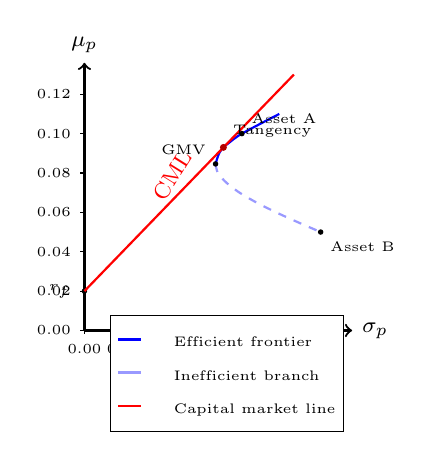
\begin{tikzpicture}[scale=0.5]
    % Axes (clipped to chart area: x in [0, 6.5], y in [0, 6.5])
    \draw[thick, ->] (0,0) -- (6.8,0) node[right] {\footnotesize $\sigma_p$};
    \draw[thick, ->] (0,0) -- (0,6.8) node[above] {\footnotesize $\mu_p$};

    % Chart border (light, optional) to visualise the plot area
    % \draw[gray!30, very thin] (0,0) rectangle (6.5,6.5);

    % Tick labels on x-axis (volatility)
    \foreach \x/\xlab in {0/0.00, 1/0.05, 2/0.10, 3/0.15, 4/0.20, 5/0.25, 6/0.30} {
        \draw (\x,0) -- (\x,-0.1);
        \node[below] at (\x,-0.1) {\tiny \xlab};
    }
    % Tick labels on y-axis (expected return)
    \foreach \y/\ylab in {0/0.00, 1/0.02, 2/0.04, 3/0.06, 4/0.08, 5/0.10, 6/0.12} {
        \draw (0,\y) -- (-0.1,\y);
        \node[left] at (-0.1,\y) {\tiny \ylab};
    }

    % Risk-free rate point on the y-axis
    \fill[black] (0,1.0) circle (2pt);
    \node[left] at (-0.1,1.0) {\tiny $r_f$};

    % Efficient frontier (upper branch of the risky-assets hyperbola).
    % Starts at GMV (w = w_GMV) and rises through the tangency portfolio
    % to asset A and beyond (short B to leverage A).
    \draw[thick, blue] plot[smooth] coordinates {
        (3.33,4.23) (3.42,4.50) (3.53,4.65) (3.65,4.75)
        (4.00,5.00) (4.95,5.50)
    };

    % Inefficient lower branch (w < w_GMV): same variance as the upper
    % branch, but lower return. Runs from GMV down-right to asset B
    % (all-B portfolio) and beyond (short A to buy more B).
    \draw[thick, blue!40, dashed] plot[smooth] coordinates {
        (3.33,4.23) (3.39,4.00) (3.61,3.75) (3.94,3.50)
        (4.37,3.25) (4.87,3.00) (5.42,2.75) (6.00,2.50)
    };

    % Capital market line: from (0, rf) through tangency, clipped at y=6.5.
    % Slope in scaled coords: (4.65-1.0)/(3.53-0) = 1.034.
    % At y=6.5: x = (6.5-1.0)/1.034 = 5.318.
    \draw[thick, red] (0,1.0) -- (5.32, 6.5);
    \node[red, above, rotate=58] at (2.6, 3.7) {\footnotesize CML};

    % Asset points
    \fill[black] (4.00,5.00) circle (2pt);
    \node[above right] at (4.00,5.00) {\tiny Asset A};
    \fill[black] (6.00,2.50) circle (2pt);
    \node[below right] at (6.00,2.50) {\tiny Asset B};

    % Global minimum-variance portfolio
    \fill[black] (3.33,4.23) circle (2pt);
    \node[above left] at (3.33,4.23) {\tiny GMV};

    % Tangency portfolio
    \fill[red!70!black] (3.53,4.65) circle (2.5pt);
    \node[above right] at (3.53,4.65) {\tiny Tangency};

    % Legend in the lower-right empty area (below the inefficient branch).
    \node[draw, fill=white, inner sep=3pt, anchor=north east]
        at (6.6, 0.4) {%
        \begin{tabular}{@{}ll@{}}
            \textcolor{blue}{\rule[0.5ex]{8pt}{1pt}} & \tiny Efficient frontier \\
            \textcolor{blue!40}{\rule[0.5ex]{8pt}{1pt}} & \tiny Inefficient branch \\
            \textcolor{red}{\rule[0.5ex]{8pt}{1pt}} & \tiny Capital market line \\
        \end{tabular}};
\end{tikzpicture}
% Coordinates: scale_x = 20 (sigma in [0, 0.30] -> 0..6 cm)
%              scale_y = 50 (mu    in [0, 0.12] -> 0..6 cm)
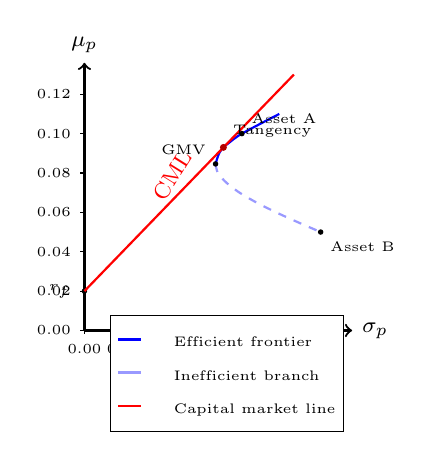
\begin{tikzpicture}[scale=0.5]
    % Axes (clipped to chart area: x in [0, 6.5], y in [0, 6.5])
    \draw[thick, ->] (0,0) -- (6.8,0) node[right] {\footnotesize $\sigma_p$};
    \draw[thick, ->] (0,0) -- (0,6.8) node[above] {\footnotesize $\mu_p$};

    % Chart border (light, optional) to visualise the plot area
    % \draw[gray!30, very thin] (0,0) rectangle (6.5,6.5);

    % Tick labels on x-axis (volatility)
    \foreach \x/\xlab in {0/0.00, 1/0.05, 2/0.10, 3/0.15, 4/0.20, 5/0.25, 6/0.30} {
        \draw (\x,0) -- (\x,-0.1);
        \node[below] at (\x,-0.1) {\tiny \xlab};
    }
    % Tick labels on y-axis (expected return)
    \foreach \y/\ylab in {0/0.00, 1/0.02, 2/0.04, 3/0.06, 4/0.08, 5/0.10, 6/0.12} {
        \draw (0,\y) -- (-0.1,\y);
        \node[left] at (-0.1,\y) {\tiny \ylab};
    }

    % Risk-free rate point on the y-axis
    \fill[black] (0,1.0) circle (2pt);
    \node[left] at (-0.1,1.0) {\tiny $r_f$};

    % Efficient frontier (upper branch of the risky-assets hyperbola).
    % Starts at GMV (w = w_GMV) and rises through the tangency portfolio
    % to asset A and beyond (short B to leverage A).
    \draw[thick, blue] plot[smooth] coordinates {
        (3.33,4.23) (3.42,4.50) (3.53,4.65) (3.65,4.75)
        (4.00,5.00) (4.95,5.50)
    };

    % Inefficient lower branch (w < w_GMV): same variance as the upper
    % branch, but lower return. Runs from GMV down-right to asset B
    % (all-B portfolio) and beyond (short A to buy more B).
    \draw[thick, blue!40, dashed] plot[smooth] coordinates {
        (3.33,4.23) (3.39,4.00) (3.61,3.75) (3.94,3.50)
        (4.37,3.25) (4.87,3.00) (5.42,2.75) (6.00,2.50)
    };

    % Capital market line: from (0, rf) through tangency, clipped at y=6.5.
    % Slope in scaled coords: (4.65-1.0)/(3.53-0) = 1.034.
    % At y=6.5: x = (6.5-1.0)/1.034 = 5.318.
    \draw[thick, red] (0,1.0) -- (5.32, 6.5);
    \node[red, above, rotate=58] at (2.6, 3.7) {\footnotesize CML};

    % Asset points
    \fill[black] (4.00,5.00) circle (2pt);
    \node[above right] at (4.00,5.00) {\tiny Asset A};
    \fill[black] (6.00,2.50) circle (2pt);
    \node[below right] at (6.00,2.50) {\tiny Asset B};

    % Global minimum-variance portfolio
    \fill[black] (3.33,4.23) circle (2pt);
    \node[above left] at (3.33,4.23) {\tiny GMV};

    % Tangency portfolio
    \fill[red!70!black] (3.53,4.65) circle (2.5pt);
    \node[above right] at (3.53,4.65) {\tiny Tangency};

    % Legend in the lower-right empty area (below the inefficient branch).
    \node[draw, fill=white, inner sep=3pt, anchor=north east]
        at (6.6, 0.4) {%
        \begin{tabular}{@{}ll@{}}
            \textcolor{blue}{\rule[0.5ex]{8pt}{1pt}} & \tiny Efficient frontier \\
            \textcolor{blue!40}{\rule[0.5ex]{8pt}{1pt}} & \tiny Inefficient branch \\
            \textcolor{red}{\rule[0.5ex]{8pt}{1pt}} & \tiny Capital market line \\
        \end{tabular}};
\end{tikzpicture}
% Coordinates: scale_x = 20 (sigma in [0, 0.30] -> 0..6 cm)
%              scale_y = 50 (mu    in [0, 0.12] -> 0..6 cm)
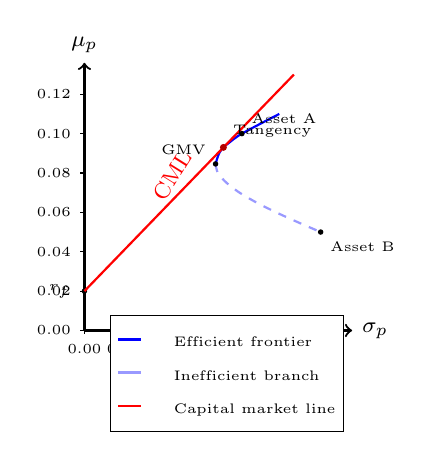
\begin{tikzpicture}[scale=0.5]
    % Axes (clipped to chart area: x in [0, 6.5], y in [0, 6.5])
    \draw[thick, ->] (0,0) -- (6.8,0) node[right] {\footnotesize $\sigma_p$};
    \draw[thick, ->] (0,0) -- (0,6.8) node[above] {\footnotesize $\mu_p$};

    % Chart border (light, optional) to visualise the plot area
    % \draw[gray!30, very thin] (0,0) rectangle (6.5,6.5);

    % Tick labels on x-axis (volatility)
    \foreach \x/\xlab in {0/0.00, 1/0.05, 2/0.10, 3/0.15, 4/0.20, 5/0.25, 6/0.30} {
        \draw (\x,0) -- (\x,-0.1);
        \node[below] at (\x,-0.1) {\tiny \xlab};
    }
    % Tick labels on y-axis (expected return)
    \foreach \y/\ylab in {0/0.00, 1/0.02, 2/0.04, 3/0.06, 4/0.08, 5/0.10, 6/0.12} {
        \draw (0,\y) -- (-0.1,\y);
        \node[left] at (-0.1,\y) {\tiny \ylab};
    }

    % Risk-free rate point on the y-axis
    \fill[black] (0,1.0) circle (2pt);
    \node[left] at (-0.1,1.0) {\tiny $r_f$};

    % Efficient frontier (upper branch of the risky-assets hyperbola).
    % Starts at GMV (w = w_GMV) and rises through the tangency portfolio
    % to asset A and beyond (short B to leverage A).
    \draw[thick, blue] plot[smooth] coordinates {
        (3.33,4.23) (3.42,4.50) (3.53,4.65) (3.65,4.75)
        (4.00,5.00) (4.95,5.50)
    };

    % Inefficient lower branch (w < w_GMV): same variance as the upper
    % branch, but lower return. Runs from GMV down-right to asset B
    % (all-B portfolio) and beyond (short A to buy more B).
    \draw[thick, blue!40, dashed] plot[smooth] coordinates {
        (3.33,4.23) (3.39,4.00) (3.61,3.75) (3.94,3.50)
        (4.37,3.25) (4.87,3.00) (5.42,2.75) (6.00,2.50)
    };

    % Capital market line: from (0, rf) through tangency, clipped at y=6.5.
    % Slope in scaled coords: (4.65-1.0)/(3.53-0) = 1.034.
    % At y=6.5: x = (6.5-1.0)/1.034 = 5.318.
    \draw[thick, red] (0,1.0) -- (5.32, 6.5);
    \node[red, above, rotate=58] at (2.6, 3.7) {\footnotesize CML};

    % Asset points
    \fill[black] (4.00,5.00) circle (2pt);
    \node[above right] at (4.00,5.00) {\tiny Asset A};
    \fill[black] (6.00,2.50) circle (2pt);
    \node[below right] at (6.00,2.50) {\tiny Asset B};

    % Global minimum-variance portfolio
    \fill[black] (3.33,4.23) circle (2pt);
    \node[above left] at (3.33,4.23) {\tiny GMV};

    % Tangency portfolio
    \fill[red!70!black] (3.53,4.65) circle (2.5pt);
    \node[above right] at (3.53,4.65) {\tiny Tangency};

    % Legend in the lower-right empty area (below the inefficient branch).
    \node[draw, fill=white, inner sep=3pt, anchor=north east]
        at (6.6, 0.4) {%
        \begin{tabular}{@{}ll@{}}
            \textcolor{blue}{\rule[0.5ex]{8pt}{1pt}} & \tiny Efficient frontier \\
            \textcolor{blue!40}{\rule[0.5ex]{8pt}{1pt}} & \tiny Inefficient branch \\
            \textcolor{red}{\rule[0.5ex]{8pt}{1pt}} & \tiny Capital market line \\
        \end{tabular}};
\end{tikzpicture}
% Coordinates: scale_x = 20 (sigma in [0, 0.30] -> 0..6 cm)
%              scale_y = 50 (mu    in [0, 0.12] -> 0..6 cm)
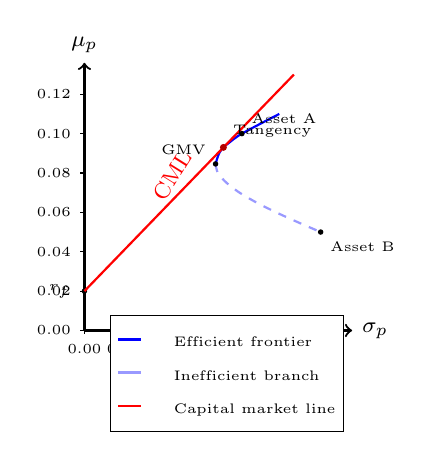
\begin{tikzpicture}[scale=0.5]
    % Axes (clipped to chart area: x in [0, 6.5], y in [0, 6.5])
    \draw[thick, ->] (0,0) -- (6.8,0) node[right] {\footnotesize $\sigma_p$};
    \draw[thick, ->] (0,0) -- (0,6.8) node[above] {\footnotesize $\mu_p$};

    % Chart border (light, optional) to visualise the plot area
    % \draw[gray!30, very thin] (0,0) rectangle (6.5,6.5);

    % Tick labels on x-axis (volatility)
    \foreach \x/\xlab in {0/0.00, 1/0.05, 2/0.10, 3/0.15, 4/0.20, 5/0.25, 6/0.30} {
        \draw (\x,0) -- (\x,-0.1);
        \node[below] at (\x,-0.1) {\tiny \xlab};
    }
    % Tick labels on y-axis (expected return)
    \foreach \y/\ylab in {0/0.00, 1/0.02, 2/0.04, 3/0.06, 4/0.08, 5/0.10, 6/0.12} {
        \draw (0,\y) -- (-0.1,\y);
        \node[left] at (-0.1,\y) {\tiny \ylab};
    }

    % Risk-free rate point on the y-axis
    \fill[black] (0,1.0) circle (2pt);
    \node[left] at (-0.1,1.0) {\tiny $r_f$};

    % Efficient frontier (upper branch of the risky-assets hyperbola).
    % Starts at GMV (w = w_GMV) and rises through the tangency portfolio
    % to asset A and beyond (short B to leverage A).
    \draw[thick, blue] plot[smooth] coordinates {
        (3.33,4.23) (3.42,4.50) (3.53,4.65) (3.65,4.75)
        (4.00,5.00) (4.95,5.50)
    };

    % Inefficient lower branch (w < w_GMV): same variance as the upper
    % branch, but lower return. Runs from GMV down-right to asset B
    % (all-B portfolio) and beyond (short A to buy more B).
    \draw[thick, blue!40, dashed] plot[smooth] coordinates {
        (3.33,4.23) (3.39,4.00) (3.61,3.75) (3.94,3.50)
        (4.37,3.25) (4.87,3.00) (5.42,2.75) (6.00,2.50)
    };

    % Capital market line: from (0, rf) through tangency, clipped at y=6.5.
    % Slope in scaled coords: (4.65-1.0)/(3.53-0) = 1.034.
    % At y=6.5: x = (6.5-1.0)/1.034 = 5.318.
    \draw[thick, red] (0,1.0) -- (5.32, 6.5);
    \node[red, above, rotate=58] at (2.6, 3.7) {\footnotesize CML};

    % Asset points
    \fill[black] (4.00,5.00) circle (2pt);
    \node[above right] at (4.00,5.00) {\tiny Asset A};
    \fill[black] (6.00,2.50) circle (2pt);
    \node[below right] at (6.00,2.50) {\tiny Asset B};

    % Global minimum-variance portfolio
    \fill[black] (3.33,4.23) circle (2pt);
    \node[above left] at (3.33,4.23) {\tiny GMV};

    % Tangency portfolio
    \fill[red!70!black] (3.53,4.65) circle (2.5pt);
    \node[above right] at (3.53,4.65) {\tiny Tangency};

    % Legend in the lower-right empty area (below the inefficient branch).
    \node[draw, fill=white, inner sep=3pt, anchor=north east]
        at (6.6, 0.4) {%
        \begin{tabular}{@{}ll@{}}
            \textcolor{blue}{\rule[0.5ex]{8pt}{1pt}} & \tiny Efficient frontier \\
            \textcolor{blue!40}{\rule[0.5ex]{8pt}{1pt}} & \tiny Inefficient branch \\
            \textcolor{red}{\rule[0.5ex]{8pt}{1pt}} & \tiny Capital market line \\
        \end{tabular}};
\end{tikzpicture}